%%%%%%%%%%%%%%%%%%%%%%%%%%%%%%%%%%%%%%%%%%%%%%%%%%%%%%%%%%%%%%%%%%%%%%%%%%%%%%%%%%%%
%Do not alter this block of commands.  If you're proficient at LaTeX, you may include additional packages, create macros, etc. immediately below this block of commands, but make sure to NOT alter the header, margin, and comment settings here. 
\documentclass[12pt]{article}
 \usepackage[margin=1in]{geometry} 
\usepackage{amsmath,amsthm,amssymb,amsfonts, enumitem, fancyhdr, color, comment, graphicx, environ}
\pagestyle{fancy}
\setlength{\headheight}{65pt}
\newenvironment{problem}[2][Problem]{\begin{trivlist}
\item[\hskip \labelsep {\bfseries #1}\hskip \labelsep {\bfseries #2.}]}{\end{trivlist}}
\newenvironment{sol}
    {\emph{Solution:}
    }
    {
    \qed
    }
\specialcomment{com}{ \color{blue} \textbf{Comment:} }{\color{black}} %for instructor comments while grading
\NewEnviron{probscore}{\marginpar{ \color{blue} \tiny Problem Score: \BODY \color{black} }}
%%%%%%%%%%%%%%%%%%%%%%%%%%%%%%%%%%%%%%%%%%%%%%%%%%%%%%%%%%%%%%%%%%%%%%%%%%%%%%%%%

\usepackage{tabto}
\usepackage{tikz}
\usepackage{tkz-berge}

%%%%%%%%%%%%%%%%%%%%%%%%%%%%%%%%%%%%%%%%%%%%%
%Fill in the appropriate information below
\lhead{Chenhao WU \\ 117010285}  %replace with your name
\rhead{Networks: Techonology, Economics and Society\\ EIE3280 Summer 2019 \\ Assignment 4} %replace XYZ with the homework course number, semester (e.g. ``Spring 2019"), and assignment number.
%%%%%%%%%%%%%%%%%%%%%%%%%%%%%%%%%%%%%%%%%%%%%

\begin{document}
	\begin{problem}{1} \textit{Computing node centrality} \\
		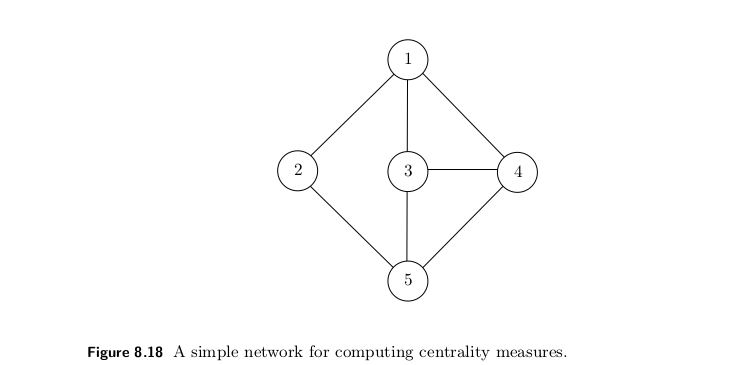
\includegraphics[width=\linewidth]{./1.png} \\
		(a). Compute the degree, closeness and eigenvector centralities of all nodes in the graph in the Figure.\\
		(b). Compute the betweenness centrality of node 2 and node 3.\\
		(c). Compute the betweenness centrality of links (3, 4) and (2, 5).
	\end{problem}
	\begin{sol}\\
		(a). \\
		First we obtain the adjacency matrix of given graph 
		\begin{align*}
			\textbf{A} &= \begin{pmatrix}0 & 1 & 1 & 1 & 0 \\ 1 & 0 & 0 & 0 & 1 \\ 1 & 0 & 0 & 1 & 1 \\ 1 & 0 & 1 & 0 & 1 \\ 0 & 1 & 1 & 1 & 0\end{pmatrix}
		\end{align*}
		From the graph one can see that the degree of node 1, 2, 3, 4 and 5 is 3, 2, 3, 3, 3, respectively. \\
		For node 1, the closeness centrality is 
		\begin{align*}
			C_1 &= \frac{5-1}{1 + 1 + 1 + 2} = \frac{4}{5} 
		\end{align*}
		For node 2, the closeness centrality is
		\begin{align*}
			C_2 &= \frac{5-1}{1+2+2+1} = \frac{2}{3}
		\end{align*}
		For node 3, the closeness centrality is
		\begin{align*}
			C_3 &= \frac{5-1}{1+2+1+1} = \frac{4}{5}
		\end{align*}
		For node 4, the closeness centrality is
		\begin{align*}
			C_4 &= \frac{5-1}{2+1+1+1} = \frac{4}{5}
		\end{align*}
		Also, by solving $Ax = \lambda x$ one can obtain the eigenvector with the highest eigenvalue of the adjacency matrix
		\begin{align*}
			x &= \begin{pmatrix}0.46 \\ 0.32 \\ 0.49 \\ 0.49 \\ 0.46\end{pmatrix}
		\end{align*}
		where x is the eigenvector centrality for each node.\\
		(b). To compute the betweenness centrality we firstly compute the matrix $G$, $N^2$ and $N^3$
		\begin{align*}
			G &= \begin{pmatrix}X & 1 & 1 & 1 & 3 \\ 1 & X & 2 & 2 & 1 \\ 1 & 2 & X & 1 & 1 \\ 1 & 2 & 1 & X & 1 \\ 3 & 1 & 1 & 1 & X\end{pmatrix} \\
			N^2 &= \begin{pmatrix}X & X & 0 & 0 & 1 \\ X & X & X & X & X \\ 0 & X & X & 0 & 0 \\ 0 & X & 0 & X & 0 \\ 1 & X & 0 & 0 & X\end{pmatrix} \\
			N^3 &= \begin{pmatrix}X & 0 & X & 0 & 1 \\ 0 & X & X & 0 & 0 \\ X & X & X & X & X \\ 0 & 0 & X & X & 0 \\ 1 & 0 & X & 0 & X\end{pmatrix}
		\end{align*}
		By the definition of betweenness centrality we can obtain that
		\begin{align*}
			B_2 &= \sum_s\sum_{t<s}\frac{n^2_{st}}{g_{st}} = \frac{1}{3} \\
			B_3 &= 
		\end{align*}
		(c). To compute the betweenness centrality of two links we firstly compute the matrix $N^{(3, 4)}$ and $N^{(2, 5)}$ respectively
		\begin{align*}
			N^{(3, 4)} &= \begin{pmatrix}X & 0 & 0 & 0 & 0 \\ 0 & X & 0 & 0 & 0 \\ 0 & 0 & X & 1 & 0 \\ 0 & 0 & 1 & X & 0 \\ 0 & 0 & 0 & 0 & X\end{pmatrix} \\
			N^{(2, 5)} &= \begin{pmatrix} X & 0 & 0 & 0 & 1 \\ 0 & X & 1 & 1 & 1 \\ 0 & 1 & X & 0 & 0 \\ 0 & 1 & 0 & X & 0 \\ 1 & 1 & 0 & 0 & X \end{pmatrix}
		\end{align*}
		By the definition of betweenness centrality we can obtain that
		\begin{align*}
			B_{(3,4)} &= \sum_s\sum_{t<s}\frac{n_{st}^{(3,4)}}{g_{st}} = 1 \\
			B_{(3,5)} &= \sum_s\sum_{t<s}\frac{n_{st}^{(2,5)}}{g_{st}} = \frac{7}{3}
		\end{align*}
	\end{sol}

	\begin{problem}{2}
		\textit{Information centrality}\\
		Consider a weighted, undirected, and connected graph with $N$ nodes, where the weight for link $(i, j)$ is $x_{ij}$. First construct a matrix $A$ where the diagonal entries $A_{ii} = 1 + \sum_j x_{ij}$, $A_{ij} = 1-x_{ij}$ if nodes $i$ and $j$ are adjacent, and $A_{ij} = 1$ otherwise. \\
		Now compute the inverse $C = A^{-1}$. The following quantity is called the information centrality of node $i$
		\begin{align*}
			C_I(i) &= \frac{1}{C_{ii}+(T-2R)/N}
		\end{align*}
		where $T = \sum_i C_{ii}$ is the trace of matrix $C$ and $R = \sum_jC_{ij}$ is any row sum of matrix $C$.\\
		Can you think of why this metric is called information centrality.
	\end{problem}
	\begin{sol}
		Let us consider a very simple case \\
		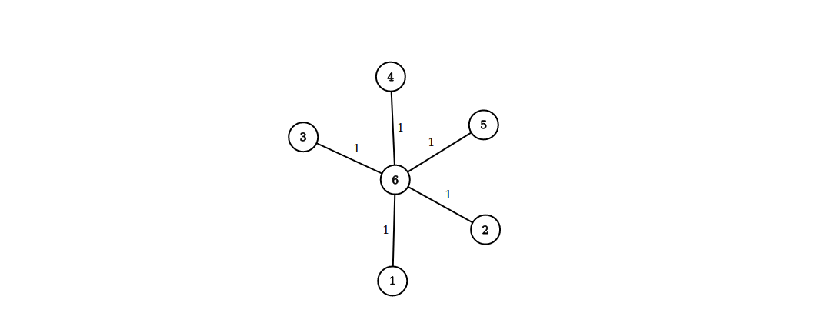
\includegraphics[width=\linewidth]{./3.png}\\
		In this case node 1, 2, 3, 4 and 5 are all connected to node 6 with equally line weight 1. First we compute the matrix $A$ by 
		\begin{align*}
			A &= \begin{pmatrix}2 & 1 & 1 & 1 & 1 & 0 \\ 1 & 2 & 1 & 1 & 1 & 0 \\ 1 & 1 & 2 & 1 & 1 & 0 \\ 1 & 1 & 1 & 2 & 1 & 0 \\ 1 & 1 & 1 & 1 & 2 & 0 \\ 0 & 0 & 0 & 0 & 0 & 6 \end{pmatrix}
		\end{align*}
		Then we calculate the inverse of $A$
		\begin{align*}
			C &= A^{-1} = \begin{pmatrix}5/6 & -1/6 & -1/6 & -1/6 & -1/6 & 0 \\ -1/6 & 5/6 & -1/6 & -1/6 & -1/6 & 0 \\-1/6 & -1/6 & 5/6 & -1/6 & -1/6 & 0 \\-1/6 & -1/6 & -1/6 & 5/6 & -1/6 & 0 \\-1/6 & -1/6 & -1/6 & -1/6 & 5/6 & 0 \\0 & 0 & 0 & 0 & 0 & 1/6\end{pmatrix}
		\end{align*}
		One can immediately notice that the sum of each row are equal to $\frac{1}{6}$ and therefore term $(T-2R)/N$ is a constant for each node, the only variable in the information centrality metric is the entries lay on the diagonal of the matrix. \\
		Then let's consider how do we compute the matrix inverse. A very general formula is $A^{-1} = \frac{1}{\det(A)}adj(A)$, where $adj(A)$ is the adjugate matrix of the origin matrix.  The computation of  the diagonal entries of the adjugate matrix can be characterized as the relative flow loss of each node, and therefore the node with higher ability to control total flows results in a less value in adjugate matrix. Then, those nodes with higher ability to control total flows will gain a higher information centrality in calculation. 
	\end{sol}

%	\begin{problem}{2}\textit{Contagion}\\
%		Consider the contagion model being run in the graph in the figure with $p = 0.3$.\\
%		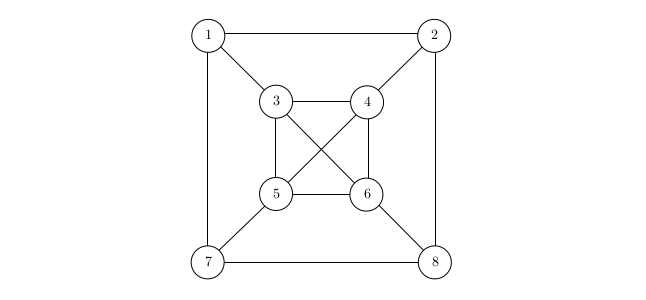
\includegraphics[width=\linewidth]{./2.png} \\
%		(a) Run the contagion model with node 1 initialized at state-1 and the other nodes initialized at state-0. \\
%		(b) Run the contagion model with node 3 initialized at state-1 and the other nodes initialized at state-0. \\
%		(c) Contrast the result from (a) and (b) and explain in terms of the cluster densities of the sets of initially state-0 nodes.
%	\end{problem}
%	\begin{sol} \\(a) Run the contagion model with initial conditions, we can obtain a table as following
%		\begin{table}[h]
%			\centering
%			\begin{tabular}{|l|l|l|}
%				\hline
%				& \textbf{state-1} & \textbf{state-0}             \\ \hline
%				\textbf{run 0} & 1       & 2, 3, 4, 5, 6, 7, 8 \\ \hline
%				\textbf{run 1} & 1, 2, 7 & 3, 4, 5, 6, 8       \\ \hline
%				\textbf{run 2} & 1, 2, 7, 8 & 3, 4, 5, 6, 7       \\ \hline
%				\multicolumn{3}{|l|}{Terminated}      \\ \hline
%			\end{tabular}
%		\end{table}\\
%		After run 2, for node 3, 4, 5 and 6, they both have equally $\frac{1}{4}$ portion of their neighborhoods that turns to state-1, thus permanently they would not flip to state-1 and the contagion model terminates at run 2.
%		\\ 
%		(b). Run the contagion model with initial conditions, we can obtain a table as following
%		\begin{table}[h]
%			\centering
%			\begin{tabular}{|l|l|l|}
%				\hline
%				& \textbf{state-1}       & \textbf{state-0}    \\ \hline
%				\textbf{run 0} & 3                      & 1, 2, 4, 5, 6, 7, 8 \\ \hline
%				\textbf{run 1} & 1, 3                   & 2, 4, 5, 6, 7, 8    \\ \hline
%				\textbf{run 2} & 1, 2, 3, 7             & 4, 5, 6, 8          \\ \hline
%				\textbf{run 3} & 1, 2, 3, 4, 5, 7, 8    & 6                   \\ \hline
%				\textbf{run 4} & 1, 2, 3, 4, 5, 6, 7, 8 &                     \\ \hline
%				terminated     &                        &                     \\ \hline
%			\end{tabular}
%		\end{table}
%		After run 4 all the nodes in the graph have flipped to state-0, thus the contagion model terminates at run 4.
%		\\
%		(c). 
%	\end{sol}
\end{document}